\documentclass{article}

\usepackage{amsmath}
\usepackage{amsfonts}
\usepackage{amssymb}

\usepackage{mathenv}

\def\nbOne{{\mathchoice {\rm 1\mskip-4mu l} {\rm 1\mskip-4mu l}
{\rm 1\mskip-4.5mu l} {\rm 1\mskip-5mu l}}}

\usepackage{vmargin}
\setmarginsrb{2.5cm}{2.5cm}{2.5cm}{2.5cm}{0cm}{0cm}{0cm}{0cm}

\usepackage[utf8]{inputenc}

\usepackage[french]{babel}
\selectlanguage{french}

\usepackage{color}
\usepackage{graphicx}
\graphicspath{{Chapitre1/}{Chapitre2/}{Chapitre3/}{Chapitre4/}} 

% Commandes personnelles %

\newcommand{\limplus}{\lim_{x\to +\infty}}
\newcommand{\limneg}{\lim_{x\to -\infty}}

\newcommand{\R}{\mathbb{R}}
\newcommand{\Z}{\mathbb{Z}}
\newcommand{\N}{\mathbb{N}}

\newcommand{\lti}{\tilde{\lambda}}
\newcommand{\mti}{\tilde{\mu}}
\newcommand{\sti}{\tilde{\sigma}}
\newcommand{\lcha}{\hat{\lambda}}
\newcommand{\mcha}{\hat{\mu}}
\newcommand{\scha}{\hat{\sigma}}
\newcommand{\gau}{\dfrac{e^\frac{-(x-\mu)^2}{2\sigma^2}}{\sqrt{2\pi\sigma^2}}}
\newcommand{\esum}[1]{\dfrac{ e^{-\sideset{}{_{i=1}^n}\sum \frac{-(x_i-#1)^2}{2\sigma^2}}} {(\sqrt{2\pi\sigma^2})^n}}
\newcommand{\sumin}{\sideset{}{_{i=1}^n}\sum}
\newcommand{\prodin}{\sideset{}{_{i=1}^n}\prod}

\definecolor{darkred}{rgb}{0.85,0,0}
\definecolor{darkblue}{rgb}{0,0,0.7}
\definecolor{darkgreen}{rgb}{0,0.7,0}
\newcommand{\dred}[1]{\textcolor{darkred}{\textbf{#1}}}
\newcommand{\dgre}[1]{\textcolor{darkgreen}{#1}}
\newcommand{\dblu}[1]{\textcolor{darkblue}{\textbf{#1}}}

\DeclareMathAlphabet{\mathpzc}{OT1}{pzc}{m}{it}

\title{\textbf{\textcolor{darkblue}{Calcul des probabilités \& théorie des erreurs.}}}
\author{\textit{Xavier Dubuc}}

\begin{document}

\maketitle

\hbox{\raisebox{0.4em}{\vrule depth 0.4pt height 0.4pt width 10cm}}

\tableofcontents % Affiche la table des matiéèes

\hbox{\raisebox{0.4em}{\vrule depth 0.4pt height 0.4pt width 10cm}}

\section*{Chapitre 0 - Introduction}

\textbf{\textcolor{darkred}{V}}ers le 1er décembre, un problème sera posé de manière individuelle et chaque étudiant devra répondre à son problème au 
travers d'un rapport (entre 20 et 50 pages) qu'il remettra à l'enseignant avant les vacances de noël. Le style est libre
mais il convient, comme dans tous rapports, de constituer celui-ci d'une introduction, d'un corps, d'une conclusion et
d'éventuellement des annexes. Il est également inutile de recopier les démonstrations du cours, un simple «comme vu au cours
à tel endroit» convient ; cependant, l'étudiant doit être capable d'expliquer la théorie cernée par cette phrase.

\textbf{\textcolor{darkred}{A}}u mois de janvier, une défense orale durant entre 10 et 30 minutes aura lieu. Au cours de celle-ci, l'étudiant sera amené à
expliquer son rapport dans le but de convaincre le jury que ce rapport a bien été fait par celui-ci. Il est à savoir que le
professeur peut demander à argumenter le choix de la méthode de résolution utilisée et ce en demandant des explications sur
une partie du cours n'étant pas spécialement utilisée dans le rapport de l'étudiant. Il convient donc de revoir tout le
cours dans son entiereté, de le comprendre et surtout d'être capable de l'appliquer.

\textbf{\textcolor{darkred}{A}}u niveau du support de cours, un syllabus est disponible au presse, son intitulé est le même que celui du cours.
Ce dernier contient la théorie inhérente au cours ainsi que des exercices et des résolutions d'exercices. Il contient
également des tables statistiques dont l'étudiant aura usage lors des séances d'exercices ainsi que 2 rapports d'anciens
élèves jugés bons à titre d'exemple pour les étudiants.

\textbf{\textcolor{darkred}{I}}l est conseillé de lire sa question dès sa réception car le problème posé peut être dur à cerner, il ne faut dès lors pas
attendre la dernière minute pour oser poser une question par rapport au problème. A cet effet, dans les environs du 8 
décembre, aura lieu une séance spéciale d'exercices durant laquelle tous les étudiants pourront poser des questions par
rapport à leur problème ainsi qu'assister à la résolution d'un exercice similaire.

\section{Chapitre 1 - 4 lois de référence}

\subsection{Loi Normale}

Prenons, par exemple, $X_i$ comme étant le temps nécessaire à produire une voiture. On a que le temps est égal à la somme
de tous les temps pour mettre chaque pièce sur la voiture (une voiture étant composée de plus ou moins 5000 pièces). On a 
donc : temps $=\sideset{}{^N_{i=1}}\sum{T_i} $. Vu $N >> 1$ ($N$ ($=5000$) est beaucoup plus grand que $1$), le 
\textbf{théorème de la limite centrale} nous dit que le temps sera de \textbf{loi normale}.

On pose : 
\begin{itemize}
 \item $X_1$ v.a.r. associée au temps d'assemblage de la 1ère voiture : mesure $x_1$.
 \item $X_2$ v.a.r. associée au temps d'assemblage de la 2ème voiture : mesure $x_2$.
 \item ...
 \item $X_i$ v.a.r. associée au temps d'assemblage de la ième voiture : mesure $x_i$.
 \item ...
 \item $X_n$ v.a.r. associée au temps d'assemblage de la nème voiture : mesure $x_n$.
\end{itemize}

$X_i$ est de loi normale, $\rightarrow f_{X_i} = \dfrac{e^{\frac{-(x-\mu)}{2\sigma^2}}}
                                                           {\sqrt{2\pi\sigma^2}}$

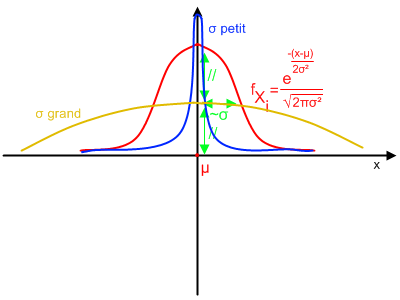
\includegraphics{Figure1-1.png}

La courbe est centrée en $\mu$ qui est la moyenne arithmétique, et la largeur (distance entre l'axe vertical passant par
$\mu$ et la courbe) à mi-hauteur est, à peu de choses près, égale à $\sigma$. On déduit les formes des courbes sur le graphe
ci-haut par le fait que vu que c'est une loi de probabilité, il faut vérifier que $\int{f(x)\ fx} = 1$ et on remarque 
également que plus $\sigma$ est petit, plus la densité est forte autour de la moyenne et plus les mesures sont précises. On
va donc toujours essayer d'avoir un $\sigma$ très petit.

Interessons nous à présent à la loi de la moyenne algébrique des v.a.r. : $\bar{X}_N = \dfrac{X_1+X_2+...+X_N}{N}$, on 
cherche donc $f_{\bar{X}_N}(x) =\ ?$. Il existe plusieurs façons de le calculer, la plus facile reste d'utiliser les 
fonctions caractéristiques. Pour $X_j$, la fonction caractéristique est donnée par : 
$\varphi_{X_j}(t) = E\{e^{itX_j}\} = e^{it\mu-\sigma^2\frac{t^2}{2}}$.

En supposant que les $X_j$ sont tous indépendants et vu qu'ils sont tous de même loi, on peut déduire les égalités
suivantes : \\
$\varphi_{\bar{X}_N}(t) \\
= E\{e^it\frac{X_1+...+X_N}{N}\} \\
= E\{e^{i\frac{t}{N}X_1+...+X_N}\} \\
= E\{e^{i\frac{t}{N} X_1}\} * E\{e^{i\frac{t}{N} X_2}\} ... E\{e^{i\frac{t}{N} X_N}\} \\
= \varphi_{X_1}\left(\frac{t}{N}\right) ... \varphi_{X_N}\left(\frac{t}{N}\right) \\
= \left(\varphi_{X_1}\left(\frac{t}{N}\right)\right)^N \\
= \left(e^ {i\frac{t}{N}\mu - \sigma^2\frac{t^2}{2N^2}} \right)^N \\
= e^{i\frac{t}{N}\mu N - \sigma^2\frac{t^2}{2N^2}N} \\
= e^{it\mu - \sigma^2\frac{t^2}{2N}} \\
= \textcolor{darkred}{e^{it\mu - \dfrac{\sigma^2}{N}\dfrac{t^2}{2}}} \\$

Nous étions entrain de considérer une loi normale de moyenne \textcolor{darkgreen}{$\mu$} et d'écart-type 
\textcolor{darkgreen}{$\sigma$}, $f_{X_i}(x) = N(\textcolor{darkgreen}{\mu},\textcolor{darkgreen}{\sigma}) \\
\Rightarrow \varphi_{X_j}(t) = e^{it\textcolor{darkgreen}{\mu}-\textcolor{darkgreen}{\sigma}^2\frac{t^2}{2}} \\ 
\Rightarrow \varphi_{\bar{X}_N}(t) = e^{it\textcolor{darkgreen}{\mu} - \textcolor{darkgreen}{\dfrac{\sigma^2}{N}}
\dfrac{t^2}{2}} = N(\mu,\dfrac{\sigma}{\sqrt{N}})$

Il s'agit donc d'une gaussienne dont l'écart-type (la largeur à mi-hauteur) est plus petit, on peut donc en conclure que
lorsque l'on considère la moyenne d'une suite d'évènements indépendants on augmente la précision des mesures. Revenons à
l'exemple de la construction de la voiture : \\
 
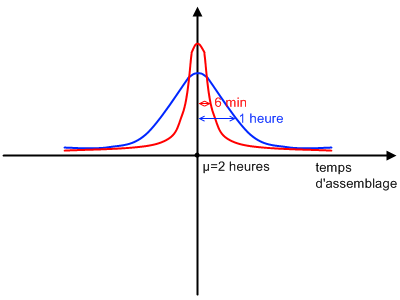
\includegraphics{Figure1-2.png}

$\textcolor{darkred}{\bar{X}_{100}} = \dfrac{X_1+...+X_{100}}{100}$ ($6$min $=$ $\dfrac{1h}{\sqrt{100}}$)

\subsection{Loi Chi 2 à $n$ degrés de liberté}

Prenons $X_i = N(0,1)$, la loi normale centrée réduite (moyenne nulle et variance 1). Il existe un moyen de «transformer»
une loi normale en une loi normale centrée réduite, imaginons que $Y$ soit une loi normale, alors $\dfrac{Y-\mu}{\sigma}$
est une loi normale centrée réduite.

On considère ensuite les «Chi 2», il s'agit en fait de la somme de toutes les mesures au carré : 
$\chi_n^2 = \sideset{}{_{i=1}^n}\sum{X_i^2}$. On donne également sa fonction de répartition : 
$f_{\chi^2_n}(x) = 
\left \{
\begin{array}{c}
 \dfrac{1}{2\Gamma(\frac{n}{2})}  (\dfrac{x}{2})^{\frac{n}{2}-1} e^{-\frac{x}{2}} \ si\ x>0\\
 0\ ailleurs
\end{array}
\right.$
Essayons de deviner l'aspect de la courbe de $f_{\chi_n^2}$, son équation est du type : $Cste\ *\ (\dfrac{x}{2})^{\frac{n}{2}-1}
e^{-\frac{x}{2}} $; on peut ainsi deviner que si $x$ est petit, on a $f_{\chi_n^2} \sim (\dfrac{x}{2})^{\frac{n}{2}-1}$ et qu'au
contraire, quand $x$ est grand, on a $f_{\chi_n^2} \sim e^{-\frac{x}{2}}$. On en déduit le graphe suivant : \\

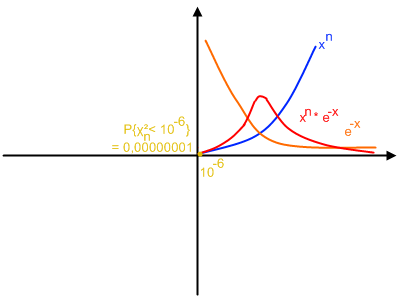
\includegraphics{Figure1-3.png}

Exemple : lors d'un labo de première année, les premières physiques ont été amené à mesurer la dilatation d'un tube de cuivre
en fonction de la température, ils ont eu une série de mesure à faire et par la suite le prof leur a dit que les points
trouvés formaient une courbe linéaire. Dès lors les élèves ont modifiés leurs graphiques afin que les points tombent sur la
droite du professeur. Cette droite est en fait la moyenne des mesures faites, et on va montrer avec l'exemple suivant que la
probabilité pour que tous les points (ici 5) se trouvent sur cette droite est infime voire nulle.

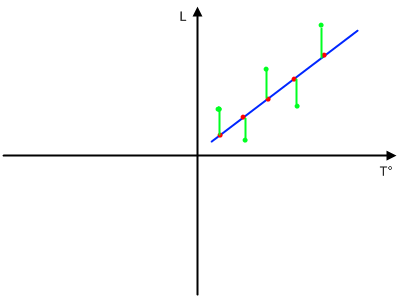
\includegraphics{Figure1-4.png}

$\sideset{}{_i}\sum{\dfrac{\left(X_i-(aT+b)\right)}{\sigma^2}} = \chi_n^2$

$\Rightarrow P\{\chi_n^2 < 10^{-6}\} = ?$

Suivons l'exemple avec $n=5$, $P\{\chi_5^2 < 10^{-6}\} = P\{0 \leq \chi_5^2 \leq 10^{-6}\} = 0,00000001$, ce qui représente
la probabilité que tous les points soient sur la droite.

La réponse la plus probable, c'est quand $\chi_n^2$ est maximum, c'est à dire aux alentours de $n$, on dit familièrement que
$\chi_n^2$ «aime» les données qui sont de l'ordre du degré de liberté.

\subsection{Loi Student à $n$ degrés de liberté}

On prend : 

$\left \{
\begin{array}{l}
X = N(0,1) \\
Y=\chi_n^2
\end{array}
\right.
$
avec $X$ et $Y$ indépendants.

On définit la loi de \textbf{Student} à $n$ degré de liberté par : $T_n = S_n = \dfrac{X}{\sqrt{\frac{Y}{n}}}$ dont la
fonction de répartition est $f_{S_n}(t) = Cste \dfrac{1}{ (1+\frac{t^2}{n}) ^ {\frac{n+1}{2}}}$

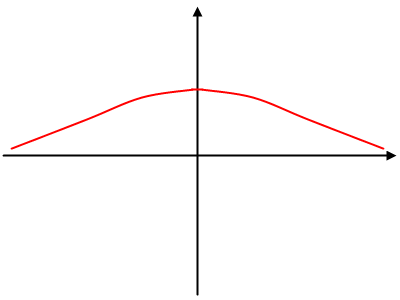
\includegraphics{Figure1-5.png}

\subsection{Loi Fisher-Snedecor à $n_1$,$n_2$ degrés de liberté}

On prend : 

$\left \{
\begin{array}{l}
X_1 = \chi_{n_1}^2 \\
X_2=\chi_{n_2}^2
\end{array}
\right.
$
avec $X_1$ et $X_2$ indépendants.

On définit la loi de \textbf{Fischer-Snedecor} à $n$ degré de liberté par : $F_{n_1,n_2} = \dfrac{\frac{X_1}{n_1}}
{\frac{X_2}{n_2}}$ dont la fonction de \indent répartition est $f(u) = 
\left \{
\begin{array}{l}
Cte \dfrac{u^{\frac{n_1}{2}} - 1} { (1 + \frac{n_1}{n_2} u) ^ {\frac{n_1+n_2}{2}}}\ \ u > 0 \\
0\ \ ailleurs.
\end{array}
\right.
$

\subsection{Résumé du chapitre 1}

\begin{tabular}{|*{4}{c|}}
\hline
\textbf{Nom de la loi} & \textbf{Symbole} & \textbf{Loi} & \textbf{Ordre des valeurs} \\
\hline
\textit{Normale} & $X_i$ & $N(0,1)$ & $\bar{X}_N$\\
\hline
\textit{Chi 2} & $\chi^2_n$ & $\sideset{}{_i^n}\sum{X_i^2}$ & De l'ordre du degré de liberté. \\
\hline
\textit{Student} & $S_n$ ou $T_n$ & $\dfrac{N(0,1)}{\sqrt{\dfrac{\chi_n^2}{n}}}$ & Autour de 0. \\
\hline
\textit{Fischer-Snedecor} & $F_{n_1,n_2}$ & $\dfrac{\chi^2_{n_1} / n_1}{\chi^2_{n_2} / n_2}$ & En général lorsque $u=1$. \\
\hline
\end{tabular} \\

\textit{Il est conseillé de connaître ce tableau et de savoir le manipuler.}

\section{Chapitre 2 - Problèmes paramétriques}

En probabilités, on utilise un modèle afin de savoir générer des nombres qui se distribuent selon la loi considérée, par 
exemple : 

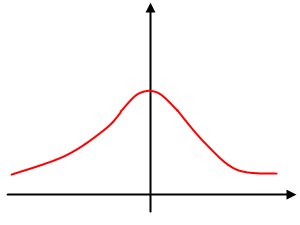
\includegraphics{Figure2-1.png}

En statistiques, on fera le chemin inverse, on aura une série de mesures et à partir de celles-ci on essayera d'appliquer
une loi. Par exemple : \\

\begin{tabular}{|*{3}{c|}}
\hline
\textbf{Jour} & \textbf{Voiture} & \textbf{Mesures} \\
\hline
\textit{Lundi} & Voiture 1 & $x_1$ secondes \\
\hline
\textit{" "} & Voiture 2 & $x_2$ secondes \\
\hline
\textit{" "} & ... & ... \\
\hline
\textit{" "} & Voiture 213 & $x_{213}$ secondes \\
\hline
\textit{Mardi} & Voiture 1 & $x'_1$ secondes \\
\hline
\textit{" "} & Voiture 2 & $x'_2$ secondes \\
\hline
\textit{" "} & ... & ... \\
\hline
\textit{" "} & Voiture 217 & $x'_{217}$ secondes \\
\hline
\end{tabular} \\

\subsection{Méthode du maximum de vraisemblance.}

A partir des mesures, on peut définir la loi de probabilité comme une fonction : $f(x,param`{e}tres)$. Pour l'instant on 
considère que l'on connaît $f$ mais on doit définir les paramètres, c'est ce que l'on appelle la statistique paramétrique.
La question que l'on se pose donc est de savoir comment trouver les paramètres à partir des mesures effectuées.

\noindent Un exemple de paramètre : $\lambda_{lundi}(x_1,x_2,x_3,...,x_{213}) = 62 min 13 sec$, \\
\indent\indent\indent\indent\indent\indent\indent\indent $\lambda_{mardi}(x'_1,x'_2,x'_3,...,x'_{217}) 
= 63 min 12 sec \rightarrow \lambda$ a un caractère aléatoire.

\noindent On va avoir recours à un estimateur pour estimer le paramètre $\lambda$, $\lcha$ : $\lcha(x_1,...,x_n)$
v.a.r. associée à $\lambda$.

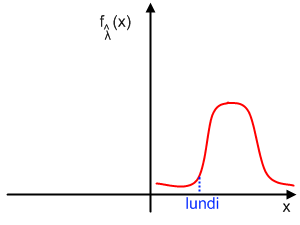
\includegraphics{Figure2-2.png}

$\rightarrow$ réalisation de l'estimateur $\lcha(X_1,...,X_n)$ (les $X_i$ sont des distributions de probabilité).\\

\noindent On pose v.a.r. de population $X = $ temps d'assemblage sur la chaîne «machin» de la voiture «truc».\\
$\rightarrow$ problème paramétrique : $f_\lambda(x,\lambda) \rightarrow$ nombre.

\noindent On va se donner un $n$-échantillons $(X_1,...,X_n)\rightarrow \lcha(X_1,...,X_n)$, on définit $L$ la
fonction de vraisemblance (on suppose que chaque expérience est semblable) par : 
$L(x_1,...,x_n,\lambda) = \sideset{}{^n_{i=1}}\prod{f_{X_i}(x_i,\lambda)}$ \\

\begin{tabular}{|*{4}{c|}}
\hline
\textbf{$1^{er}$ Jour} & \textbf{$2^{`eme}$ Jour} & ... & \textbf{$K^{`eme}$ Jour} \\
\hline
$x_1$ & $x'_1$ & ... & $x_1^{(k)}$ \\
\hline
... & ... & ... & ...\\
\hline
$x_n$ & $x'_m$ & ... & $x_p^{(k)}$ \\
\hline
$\lti$($x_1$,...,$x_n$) & $\lti$($x'_1$,...,$x'_m$) & ... & $\lti$($x_1^{(k)}$,...,$x_p^{(k)}$) \\
\hline
\end{tabular} \\

$\rightarrow$ histogramme des $\lti$ : \\

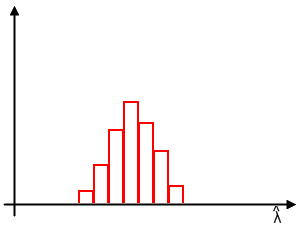
\includegraphics{Figure2-3.png}

\underline{Propriétés} : \\

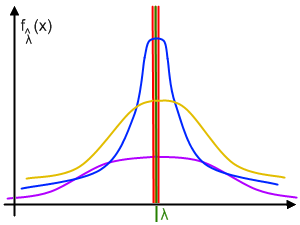
\includegraphics{Figure2-4.png}

On veut que $E(\lambda$\^{}$) = \lambda$, c'est la propriété de l'estimateur \textbf{non-biaisé}.\\
La courbe bleue signifie que les résultats sont fort proches $\Rightarrow$ minimisation de l'erreur. \\
La courbe violette signifie que les résultats sont fort espacées $\Rightarrow$ maximisation de l'erreur. \\
La courbe orange/rouge est impossible, on va le prouver : \\

\underline{Inégalité de Rao-Cramer-Freschet} \\

$\forall u$ réel, on pose $g(u) = ( u (\lti-\lambda ) + \delta_\lambda\log{(L)} )$, on a : $\forall u \in \R,
g^2(u) \geq 0 $ et on va prouver : $E \{g^2(u)\} \geq 0$. \\

$E \{g^2(u)\} \geq 0 \\
\Leftrightarrow E\{u^2 (\lti-\lambda)^2 + 2u (\lti-\lambda) \delta_\lambda\log{(L)}
+ (\delta_\lambda\log{(L)}^2 \} \geq 0\\
\Leftrightarrow u^2 E \{ (\lti-\lambda) \} + 2u E\{(\lti-\lambda) \delta_\lambda\log{(L)} \}
+ E \{ (\delta_\lambda\log{(L)})^2 \} \geq 0 \\
\Leftrightarrow u^2\sigma^2(\lti) + 2u E\{(\lti-\lambda) \delta_\lambda\log{(L)} \} + E \{ (\delta_\lambda\log{(L)})^2 \}
\geq 0 \\$
Soit à simplifier : $E\{(\lti-\lambda) \delta_\lambda\log{(L)} \} = E \{ \lti \dfrac{\delta_\lambda(L)}{L} \}
- \lambda E\{\dfrac{\delta_\lambda(L)}{L}\}$ \\ 
\textit{(dérivée d'un log par rapport à une variable = dérivée de la variable / variable)} \\
$E \{ \lti \dfrac{\delta_\lambda(L)}{L} \} \\
= \int dx_1 ... \int dx_n \lti(x_1...x_n) \dfrac{\delta_\lambda(L)}{L} \sideset{}{_i}\prod{(f(X_i,\lambda))} \\
= \delta_\lambda (\lambda)$ \textit{(car sans biais)} \\
$= 1$ \\

\noindent $ \lambda E\{\dfrac{\delta_\lambda(L)}{L}\}\\
= \int dx_1 ... \int dx_n \dfrac{\delta_\lambda(L)}{L} \sideset{}{_i}\prod{(f(X_i,\lambda))} \\ 
= \delta_\lambda \int dx_1 ... \int dx_n L(x_1,...,x_n,\lambda) \\
= \delta_\lambda (1) \\
= 0$

$\rightarrow E\{g^2(x)\} = u^2\sigma^2(\lti + 2u + E \{ (\delta_\lambda\log{(L)})^2 \} \geq 0\ \forall u \in \R \\
\rightarrow = du^2+bu+c \\$

\begin{tabular}{|*{5}{c|}}
\hline
... & $u_1$ & ... & $u_2$ & ... \\
\hline
$+$ & $0$ & $-$ & $+$ & $0$ \\
\hline
\end{tabular} \\

Il ne peut y avoir 2 racines réelles distinctes car $\geq 0\ \forall u$, donc le discriminant $\Delta \leq 0$. \\
$\Delta = 4 - 4 \sigma^2(\lti) E\{ (\delta_\lambda\log{(L)})^2 \} \leq 0 \\ 
\Leftrightarrow 1 - \sigma^2(\lti) E\{ (\delta_\lambda\log{(L)})^2 \} \leq 0 \\ 
\Leftrightarrow 1 \leq \sigma^2(\lti) E\{ (\delta_\lambda\log{(L)})^2 \} \\ 
\Leftrightarrow 0 < \dfrac{1}{E\{ (\delta_\lambda\log{(L)})^2 \}} \leq \sigma^2(\lambda$\~{}$) \\ 
\rightarrow$ la variance ne vaudra jamais 0 $\rightarrow \sigma > 0$, ce qui implique que la courbe rouge est impossible et que
donc un estimateur sans erreur est impossible.

\subsubsection*{Construire des estimateurs}

On veut un estimateur \textbf{efficace}, c'est-à-dire un estimateur :
\begin{itemize}
\item sans biais : $ E(\lti) = \lambda$
\item de variance minimale : $\sigma^2(\lti) = \dfrac{1}{E\{(\delta_\lambda\log{(L)})^2 \}}$
\end{itemize}

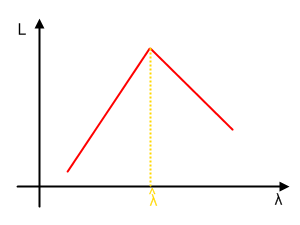
\includegraphics{Figure2-5.png}

\noindent \underline{Méthode $\lti $ ?} \\

\noindent $L(\textcolor{darkgreen}{x_1,...,x_n},\lambda)$ \textcolor{darkgreen}{mesures réalisées, elles sont donc connues}.\\
$\lambda$\^{} estimateur dont la réalisation $\lti$ réalise le maximum de $L(x_1,...,x_n,\lambda)$. \\

\noindent\underline{Exemple} : \underline{$\lcha = $ chaîne d'assemblage de voitures} \\
Population $\lambda$ : $f_X(x) = \dfrac{e^{(-x-\mu)^2 / 2\sigma^2}}{\sqrt{2\pi\sigma^2}}$
$\rightarrow$ on dit que $\sigma^2 = \sigma_0^2$ (on le fixe), \\
$\rightarrow f_X(x) = \dfrac{e^{(-x-\mu)^2 / 2\sigma_0^2}}{\sqrt{2\pi\sigma_0^2}} $ \\
$\mcha$ ? $\rightarrow \mcha$($x_1,...,x_n$) \\
$\rightarrow \sideset{}{_1^n}\prod{f(x_i,\mu)} \\ 
= \sideset{}{_1^n}\prod{\dfrac{e^{(-x_i-\mu)^2 / 2\sigma_0^2}}{\sqrt{2\pi\sigma_0^2}}} \\
= \dfrac{e^{-\sideset{}{_{i=1}^n}\sum(x_i-\mu)^2 / 2\sigma_0^2}} {\sqrt{2\pi\sigma_0^2}}$ \\
$\mu$ ? maximum $L \rightarrow \mu$ ? maximum $\log{(L)}$ (car log est une fonction monotone croissante) \\
$\log{(L)} = -\sideset{}{_{i=1}^n}\sum{(x_i-\mu)^2 / 2\sigma_0^2} - \dfrac{n}{2} \log{(2\pi\sigma_0^2)}$ \\
$\rightarrow \delta_N\log{(L)} |_{\mu = \mti_n} = 0$ \textit{(Equation de vraisemblance)}. \\
$\Leftrightarrow \sideset{}{_i^n}\sum\dfrac{2(x_i-\mti)}{2\sigma_0^2} - 0 = 0$ \\
$\Leftrightarrow \sideset{}{_{i=1}^n}\sum{(x_i-\mti)} = 0 \\
\Leftrightarrow \sideset{}{_{i=1}^n}\sum{(x_i)} - n\mti = 0 \\
\Leftrightarrow \mti = \dfrac{1}{n} \sideset{}{_{i=1}^n}\sum{(x_i)} \\
\Leftrightarrow \mti(x_1,...,x_n) = \dfrac{1}{n}\sideset{}{_{i=1}^n}\sum{(x_i)} = \bar{x}_n$
%~ les mu dans les 4 dernières lignes sont des mu^~

\noindent On peut faire pareil en fixant $\mu = \mu_0$ et en cherchant $\sigma^2$, on trouve : 
$\sigma^2 = \dfrac{1}{n} \sideset{}{_{i=1}^n}\sum{(x_i-\mu_0)^2}$

\noindent Imaginons que l'on ne connait rien, on a $f_X(x,\mu,\sigma^2) =
\dfrac{e^{(-x-\mu)^2 / 2\sigma^2}}{\sqrt{2\pi\sigma^2}}$ \\
$L =  \dfrac{e^{-\sideset{}{_{i=1}^n}\sum(x_i-\mu)^2 / 2\sigma_0^2}} {\sqrt{2\pi\sigma_0^2}} \\
\Leftrightarrow \log{(L)} = - \sideset{}{_{i=1}^n}\sum \left((x_i-\mu)^2 / 2\sigma^2\right) \\$
On aura max $\log{(L)}$ uniquement lorsque : \\

\[
 \left \{
 \begin{array}{c @{ = } c c}
   \delta_{\mti} \log{(L)} |_{\mti ,\scha^{2}} & 0 & \textcolor{darkred}{(1)} \\
   \delta_{\scha^ 2} \log(L) |_{\mti ,\scha ^2} & 0 & \textcolor{darkgreen}{(2)}\\
 \end{array}
 \right.
\]

\textcolor{darkred}{(1)}$= + 2\sideset{}{_{i=1}^n}\sum \dfrac{(x_i-\mti)}{2\sti^2} \\
\rightarrow \sideset{}{_{i=1}^n}\sum (x_i-\mti) = 0 \\
\Leftrightarrow \sideset{}{_{i=1}^n}\sum (x_i) - n \mti = 0 \\
\Leftrightarrow \mti = \dfrac{1}{n} \sideset{}{_{i=1}^n}\sum (x_i) = \bar{x}_n \\
\Leftrightarrow \boxed{\mcha = \dfrac{1}{n} \sideset{}{_{i=1}^n}\sum (X_i) = \bar{X}_n} \\$

\textcolor{darkgreen}{(2)} $= + \sideset{}{_{i=1}^n}\sum \dfrac{(x_i-\mti)^2}{2(\sti^2)^2} - \dfrac{n}{2\sti^2} \\
\rightarrow \sti^2 = \dfrac{1}{n} \sideset{}{_{i=1}^n}\sum (x_i-\mti)^2 \\
\Leftrightarrow \boxed{\scha^2 = \dfrac{1}{n} \sideset{}{_{i=1}^n}\sum (X_i-\bar{X}_n)^2}$ \\


\noindent \underline{Motivations} \textit{(pour utiliser cette méthode)}

\begin{enumerate}
\item Si, dans un problème donné $f_X(x,\lambda)$, il existe un estimateur efficace ; \textbf{alors} il est solution de
l'équation de vraisemblance.
\item Si, dans un problème donné $f_X(x,\lambda)$, il \textbf{n'}existe \textbf{pas} un estimateur efficace ; \textbf{alors}
la méthode du maximum de vraisemblance en fournit un qui devient asymptotiquement ($n\to\infty$) efficace. \\

$\rightarrow \dfrac{\lcha - \lambda}{\sqrt{var\ .\ min}} = \dfrac{\lcha - \lambda}{\sqrt{E\{(\delta_\lambda \log{(L)})^2\}}}
 \rightarrow_{n\to\infty} N(0,1)$ \\
\end{enumerate}

On a donc, dans l'exemple plus haut, calculer les 2 paramètres de $f(x,\lambda_1,\lambda_2)$ constituant le modèle d'une série
de données que l'on nous a donné (avec $f$ connue). \\ On avait donc comme données de départ : $x$ ainsi que 
$f(x,\lambda_1,\lambda_2) = \dfrac{e^{\dfrac{-(x-\lambda_1)^2}{2\lambda_2^2}}}{\sqrt{2\pi\lambda_2^2}}$. \\ On a ensuite montré
que $\lcha_1 = \dfrac{1}{n} \sideset{}{_{i=1}^n}\sum X_i$ \& $\lcha_2 = \dfrac{1}{n} 
\sideset{}{_{i=1}^n}\sum(X_i-\bar{X}_n)^2$. \\

\noindent\underline{Autre exemple} : \underline{Temps d'attente entre 2 coups de téléphone.} \textit{(Loi de Poisson)}

\noindent P$\{X=k\} = e^{-\lambda} \dfrac{\lambda^k}{k!} \rightarrow$ paramètre $\lambda$. \\
n-échantillons : $(x_1\ ...\ x_n) \rightarrow \lcha$ ? $\rightarrow \dfrac{\delta}{\delta\lambda} \log{(L)} 
|_{\lambda=\lcha} = 0$.

\subsection{Méthode d'estimation par intervalle}

$N:N(0,1) \rightarrow P\{ -a < N < +a \} = \sideset{}{_{-a}^{+a}}\int f_N(x)dx = 
\sideset{}{_{-a}^{+a}}\int \dfrac{e^{-\frac{x^2}{2}}}{\sqrt{2\pi}} dx= 
2 \sideset{}{_{0}^{a}}\int \dfrac{e^{-\frac{x^2}{2}}}{\sqrt{2\pi}} dx$

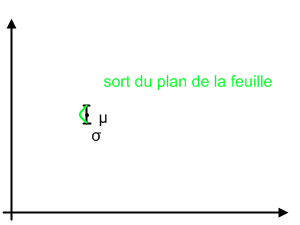
\includegraphics{Figure2-6.png}

\underline{Exemple} : 
\begin{itemize}
\item 1 déviation standard : $P\{ -1 < \dfrac{X-\mu}{\sigma} < +1 \} = 2P\{0<N<1\} = 2 * 0,3413 = 0,6826$
$\rightarrow$ pratiquement $\dfrac{2}{3}$ chances qu'on tombe dans la barre d'erreur, $\dfrac{1}{3}$ des points seront en
dehors.
\item 3 déviations standards : $P\{ -3 < \dfrac{X-\mu}{\sigma} < +3 \} = 2 * 0,4987 = 0,998 \rightarrow \dfrac{2}{1000}$ points
en dehors.
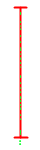
\includegraphics{Figure2-7.png}
\end{itemize}

$X_1$ : Gaussienne : $N(\mu,\sigma) \rightarrow \bar{X}_n = \dfrac{1}{n}\sideset{}{_i}\sum X_i = N(\mu,\sigma/\sqrt{n})$ \\
\indent $\Rightarrow \dfrac{\bar{X}_n - \mu}{\sigma/\sqrt{n}} : N(0,1)$

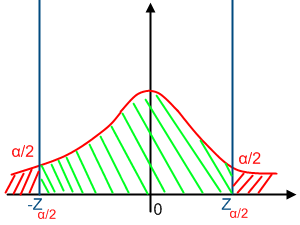
\includegraphics{Figure2-8.png}

$P \{ -Z_{\frac{\alpha}{2}} < \dfrac{\bar{X}_n - \mu}{\sigma/\sqrt{n}} < Z_{\frac{\alpha}{2}} \} = 1 - \alpha$ 

\underline{$\sigma$ connu} : \\

$P \{ -Z_{\frac{\alpha}{2}} \dfrac{\sigma}{\sqrt{n}} < \bar{X}_n - \mu < Z_{\frac{\alpha}{2}} \dfrac{\sigma}{\sqrt{n}}\}
= 1 - \alpha$ \\ 
\indent $P \{ \bar{X}_n - Z_{\frac{\alpha}{2}} \dfrac{\sigma}{\sqrt{n}} < \mu < \bar{X}_n + Z_{\frac{\alpha}{2}} 
\dfrac{\sigma}{\sqrt{n}}\} = 1 - \alpha$ \\ 

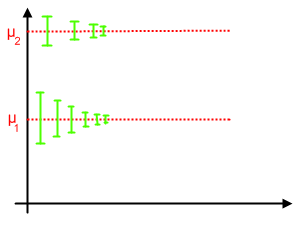
\includegraphics{Figure2-9.png}

\underline{Estimation par intervalle} $\rightarrow$ on veut $\mu$ avec une précision donnée.

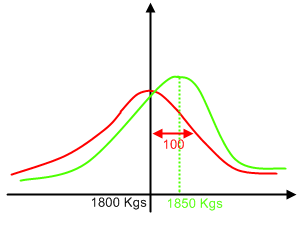
\includegraphics{Figure2-10.png}

\subsubsection{Tests d'hypothèse}

\underline{Exemple} : \textit{Charge de rupture : 1800 kgs}, on utilise un nouveau procédé $\rightarrow$ meilleurs cables 
$\rightarrow$ échantillons de $50$ nouveaux câbles.

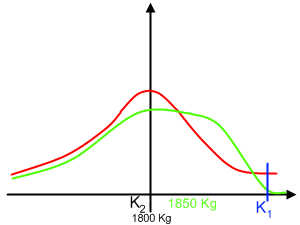
\includegraphics{Figure2-11.png}

\noindent $(x_1,...,x_n)^2$ $\rightarrow \boxed{\bar{X}_n > K}$ ? ($\rightarrow$ nouveau procédé) \\
\noindent $\bar{X}_n \leq K$ ($\rightarrow$ ancien procédé)

\begin{tabular}{|*{4}{c|}}
\hline
$K_1$ & ancien procédé & nouveau procédé & $K_2$  \\
\hline
accepte sur base du test & rejet de l'ancien procédé (1) & (2) & (3)\\
\hline
rejette sur base du test & . & (4) & (5)\\
\hline
\end{tabular} \\

$(x_1,...,x_{50}) \rightarrow$ modèle ? 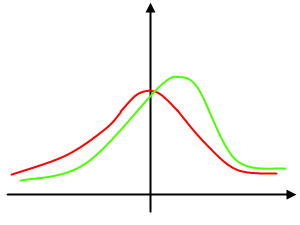
\includegraphics{Figure2-12.png}

$H_0 = H_1^c$, $H_1 = H_0^c$ \\

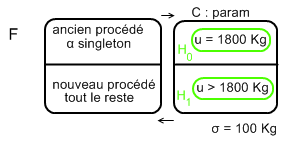
\includegraphics{Figure2-13.png}

\noindent $H_0 \rightarrow AH_0$ \\
\indent $\rightarrow RH_0 = P\{$Rejet $H_0$ alors que $H_0$ est vrai$\}$ \\
$H_1 \rightarrow AH_1$ \\
\indent $\rightarrow RH_1 = P\{$Rejet $H_1$ alors que $H_1$ est vrai$\}$ \\

\begin{tabular}{|*{3}{c|}}
\hline
$\rightarrow$ & $H_0$ & $H_1$  \\
\hline
$RH_0$ & $\alpha$ : erreur de $1^{ere}$ espèce & \textcolor{darkgreen}{V} \\
\hline
$RH_1$ & \textcolor{darkgreen}{V} & $\beta$ : erreur de $2^{eme}$ espèce\\
\hline
\end{tabular} \\

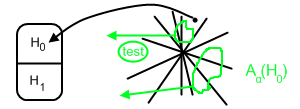
\includegraphics{Figure2-14.png}

$P\{RH_0/H_0\} = \alpha$, $P\{RH_1/H_1\} = \beta$ \\

$H_0$, $\alpha$ \& $\beta$, $T_1$ est plus puissant que $T_2$ ssi $\alpha_1 \leq \alpha_2$ \& $\beta_1 \leq \beta_2$ \\

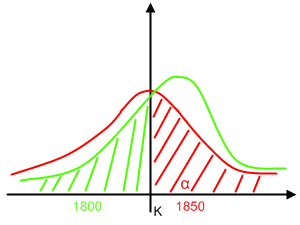
\includegraphics{Figure2-15.png}

\begin{tabular}{|*{4}{c|}}
\hline
Cas & $H_0$ & $H_1$ & Méthode\\
\hline
1) & simple & simple & Neyman-Pearson \\
\hline
2) & simple & composé & méthode du quotient de vraisemblance\\
\hline
3) & composé & simple & méthode du quotient de vraisemblance\\
\hline
4) & composé & composé & méthode du quotient de vraisemblance\\
\hline
\end{tabular} \\

\noindent H simple : $\{singleton\} \subset H$ (espace des paramètres), $F$ : Gaussienne$(\mu,\sigma^2)$ \\
H composé : le contraire.

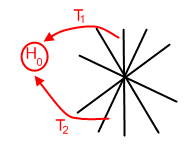
\includegraphics{Figure2-16.png}
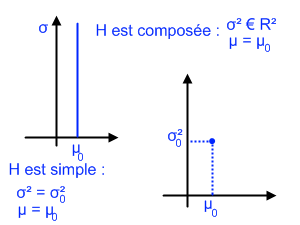
\includegraphics{Figure2-18.png}

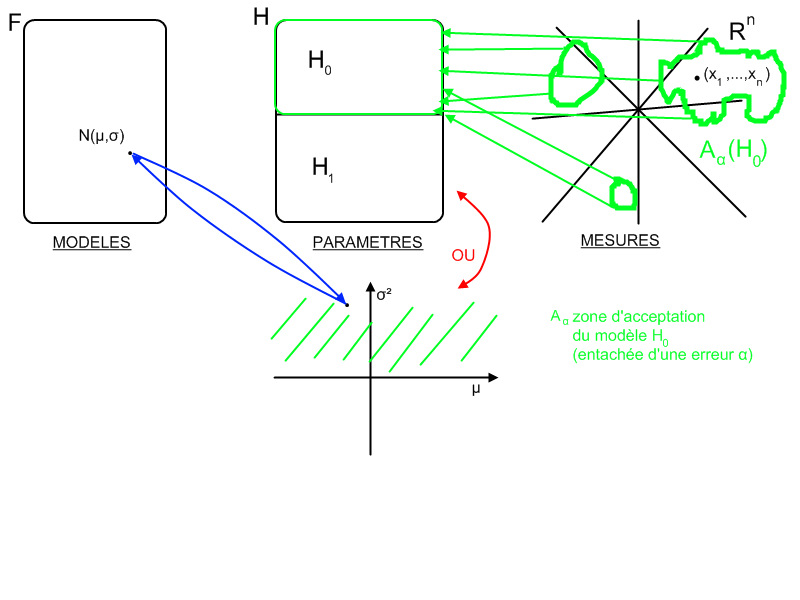
\includegraphics[width=500px]{Figure2-17.png}
\subsubsection{Théorème de Neyman-Pearson}

\noindent On prend une population $f(x,\theta)$ avec $\theta\in\{\theta_1,\theta_2\}$ \textit{(espace des paramètres)}.\\
On se donne un $n$-échantillons $(X_1,...,X_n)$ qui réalise des mesures ($x_1,...,x_n)$. \\
On construit la fonction de vraisemblance : $L(x_1,...,x_n,\theta) = \sideset{}{_{i=1}^n}\prod f(x_i,\theta)$. \\

Hypothèses : $H_0 : \theta = \theta_1$ ; $H_1 : \theta = \theta_2$ \\

Le théorème dit alors : 

\begin{enumerate}
\item $\forall \alpha$(risque de première espèce) $\in [0,1] \exists C_\alpha \geq 0$ tel que $A_\alpha = 
\{ (x_i...x_n) \in \R^n | \dfrac{L(x_1,...,x_n,\theta_1}{L(x_1,...,x_n,\theta_2} \leq C_\alpha \}$ vérifie 
$P_{H_0}(A_\alpha) = 1-\alpha$
\item Le test admettant $A_\alpha$ comme zone d'acceptation est le plus puissant (minimise l'erreur de 2ème espèce $\beta$).
\end{enumerate}

\noindent\underline{Exemple} : Cartes réseau.

\noindent On a le choix entre 2 type de carte : $\mu_0 = 10$Gb/s ; $\mu_1 = 20$Gb/s ; on fixe $sigma^2_0 = \sigma^2_0 = 1$Mb/s.
On connait la fonction de répartition : $f_X(x) = \gau$.

\noindent $L(x_1,...,x_n,\mu,\sigma^2) = \sideset{}{^n_{i=1}}\prod f_{X_i}(x_i) \\
= \sideset{}{^n_{i=1}}\prod\dfrac{e^\frac{-(x_i-\mu)^2}{2\sigma^2}}{\sqrt{2\pi\sigma^2}}\\
= \esum{\mu}$ 

$\dfrac{L(x_1,...,x_n,\mu_0,\sigma_0^2)}{L(x_1,...,x_n,\mu\sigma_0^2)} \\
= \dfrac{\esum{\mu_0}}{\esum{\mu_1}} \\
= \dfrac{e^{-\sumin \frac{(x_i - \mu_0)^2}{2\sigma_0^2} }} {e^{-\sumin \frac{(x_i - \mu_1)^2}{2\sigma_0^2} }} \\
= e^{-\sumin \frac{(x_i - \mu_0)^2}{2\sigma_0^2} } {e^{+\sumin \frac{(x_i - \mu_0)^2}{2\sigma_0^2} }}$
($\dfrac{1}{e^{-a}} = e^{+a}$) \\ $
= e^{-\frac{1}{2\sigma_0^2} \left\{ \sumin(x_i-\mu_0)^2 - \sumin(x_i-\mu_1)^2 \right\} } \\
= e^{-\frac{1}{2\sigma_0^2} \left\{ \sumin(x_i^2) - 2\mu_0\sumin(x_i) + \sumin(\mu_0^2) - \sumin(x_i^2)
+ 2\mu_1\sumin(x_i) - \sumin(\mu_1^2) \right\} } \\
= e^{-\frac{1}{2\sigma_0^2} \left\{ 2(\mu_1-\mu_0)\sumin(x_i) + n(\mu_0^2-\mu_1^2) \right\} } \\$

Par Neyman-Pearson, $\exists C_\alpha$ tq $P_{H_0}\{ e^{...} \leq C_\alpha\} = 1-\alpha$ \\
(On fixe le fait qu'on accepte un risque de $\alpha = 10\%$, dès lors si on examine l'égalité, on connait tout sauf $C_\alpha$.)\\
$ $ \\

\begin{tabular}{l}
\hline
\noindent\underline{Rappel} : \textit{Chapitre 1}\\ 
$X_1$ : gaussienne : $N(\mu_0,\sigma_0) \rightarrow \sumin (X_i)/n = \bar{X}_n$ \\
$\bar{X}_n$ : $N(\mu_0,\frac{\sigma_0}{n}) \Rightarrow \dfrac{\bar{X}_n-\mu_0}{\frac{\sigma_0}{n}}$ : $N(0,1)$ \\
\hline
\end{tabular} \\

$ $ \\

\noindent $\Rightarrow P_{H_0} \left\{ \dfrac{-1}{2\sigma_0^2} ... \leq \log C_\alpha (=C_\alpha') \right\} = 1-\alpha\\
\Leftrightarrow P_{H_0} \left\{ (x_1,...,x_n) \in \R^N | - \dfrac{2}{2\sigma_0^2} 
(\mu_1 -\mu_0) \sumin (x_i) \leq C_\alpha '' \right\} = 1-\alpha$ (but : se ramener à une loi du premier chapitre) $ \\
\Leftrightarrow P_{H_0} \left\{ n \dfrac{\mu_0 - \mu_1}{\sigma_0^2} \dfrac{1}{n} \sumin x_i \leq C_\alpha'' \right\} = 1-\alpha$
(on multiplie par $n$ et on divise par $n$) \\ $
\Leftrightarrow P_{H_0} \left\{ \dfrac{\mu_0 - \mu_1}{\frac{\sigma_0^2}{n}} \bar{X}_n \leq C_\alpha'' \right\} = 1-\alpha$
\begin{enumerate}
\item \underline{$\mu_0>\mu_1$} $\rightarrow$ $P_{H_0} \left\{ \dfrac{\bar{X}_n - \mu_0}{\sigma_0/\sqrt{n}} \leq 
C_\alpha'''\right\} = 1-\alpha$ (ici, par les tables, $C_\alpha''' = 1,28$) \\

\item \underline{$\mu_1>\mu_0$} $\rightarrow$ $P_{H_0} \left\{ \dfrac{\bar{X}_n - \mu_0}{\sigma_0/\sqrt{n}} \geq 
C_\alpha'''\right\} = 1-\alpha$ (ici, par les tables, $C_\alpha''' = 1,28$) \\

\end{enumerate}

\subsubsection{Méthode du quotient de vraisemblance}

On introduit $\Lambda_n = \dfrac{\sup_HL}{\sup_{H_0}L}$ et on dit qu'on est : 
\begin{itemize}
\item dans la zone \textbf{d'acceptation} si $P\{\Lambda_n \leq \lambda_\alpha\} = 1-\alpha$
\item dans la zone \textbf{de rejet} si $P\{\Lambda_n > \lambda_\alpha \} = \alpha$
\end{itemize}

\noindent \underline{Exemple} : (voir syllabus p70) \\
On prend une population Gaussienne, et on a 2 hypothèses : $H_0 : \mu = \mu_0$ et $H_1 : \mu \neq \mu_O$. \\
On construit la fonction de vraisemblance : $\prodin \gau = \esum{\mu}$. \\
\underline{numérateur} : $\sup_HL = sup_{(\mu,\sigma^2)}L = L(x_1...x_n,\mcha,\scha^2)$ \\
\indent avec $\mcha = \dfrac{1}{n}\sumin x_i$ et $\scha^2 = \dfrac{1}{n} \sumin (x_i-\mcha)^2$ \\
\underline{dénominateur} : $\sup_HL = sup_{(\mu=\mu_0,\sigma^2)}L = L(x_1...x_n,\mu_0,\scha^2_2)$ \\
\indent avec $\scha^2_2 = \dfrac{1}{n} \sumin (x_i-\mu_0)^2$ \\

$\Rightarrow \Lambda_n = \frac{numerateur}{denominateur} \\
= \dfrac{L(x_1...x_n,\mcha,\scha^2)}{L(x_1...x_n,\mu_0,\scha^2_2)}
= \dfrac{ \dfrac{e^{-\sumin\dfrac{(x_i-\bar{x}_n)^2}
		{2 \left( \frac{1}{n} \sumin (x_i-\bar{x}_n)^2 \right)  }}}
		{\left(\sqrt{\dfrac{2\pi}{n} \sumin (x_i-\bar{x}_n)^2}\right)^n} }
		% Denominateur
		{ \dfrac{e^{-\sumin\dfrac{(x_i-\mu_0)^2}
		{2 \left( \frac{1}{n} \sumin (x_i-\mu_0)^2 \right)  }}}
		{\left(\sqrt{\dfrac{2\pi}{n} \sumin (x_i-\mu_0)^2}\right)^n}}
$ \\
Les $e^{-...}$ se neutralisent car se simplifient toutes les 2 en $e^{n/2} \\
= \left(\dfrac{\sumin (x_i-\mu_0)^2}{\sumin (x_i-\bar{x}_n)^2}\right)^{n/2} \\$

A faire donc : $P\left\{ A_\alpha | \left(\dfrac{\sumin (x_i-\mu_0)^2}{\sumin (x_i-\bar{x}_n)^2}\right)^{n/2} 
\leq \lambda_\alpha \right\} = 1-\alpha \\
\Leftrightarrow P\left\{ A_\alpha | \left(\dfrac{\sumin (x_i-\mu_0)^2}{\sumin (x_i-\bar{x}_n)^2}\right) 
\leq (\lambda_\alpha)^{2/n} = \lambda_\alpha' \right\} = 1-\alpha \\
\Rightarrow $ Se ramener à une loi du chapitre 1. \\

\noindent \underline{On cherche à simplifier} : \\

$\left(\dfrac{\sumin (x_i-\mu_0)^2}{\sumin (x_i-\bar{x}_n)^2}\right) \\
= \left(\dfrac{\sumin (x_i-\bar{x}_n+\bar{x}_n-\mu_0)^2}{\sumin (x_i-\bar{x}_n)^2}\right) \\
= \dfrac{\sumin(x_i-\bar{x}_n)^2 + 2 (\bar{x}_n-\mu_0)\sumin(x_i-\bar{x}_n) + n(\bar{x}_n-\mu_0)^2}
		{\sumin (x_i-\bar{x}_n)^2} \\ 
= \dfrac{\sumin(x_i-\bar{x}_n)^2 + \left[2 (\bar{x}_n-\mu_0)\left(\sumin(x_i)-\sumin\bar{x}_n\right) \right] + 
n(\bar{x}_n-\mu_0)^2}		{\sumin (x_i-\bar{x}_n)^2} \\ 
= \dfrac{\sumin(x_i-\bar{x}_n)^2 + \left[2 (\bar{x}_n-\mu_0)\left(\sumin(x_i)-n\bar{x}_n\right) \right] + 
n(\bar{x}_n-\mu_0)^2}		{\sumin (x_i-\bar{x}_n)^2} \\ 
= \dfrac{\sumin(x_i-\bar{x}_n)^2 + \left[2 (\bar{x}_n-\mu_0)\left(\sumin(x_i)-n\frac{1}{n}\sumin(x_i)\right) \right] + 
n(\bar{x}_n-\mu_0)^2}		{\sumin (x_i-\bar{x}_n)^2}$ (par définition de $\bar{x}_n$)$\\ 
= \dfrac{\sumin(x_i-\bar{x}_n)^2 + \dred{0} + n(\bar{x}_n-\mu_0)^2}		{\sumin (x_i-\bar{x}_n)^2} \\ 
= 1 + \dfrac{n(\bar{x}_n-\mu_0)^2} {\sumin (x_i-\bar{x}_n)^2} \\ 
\Rightarrow P\left\{ A_\alpha | \dfrac{n(\bar{x}_n-\mu_0)^2} {\sumin (x_i-\bar{x}_n)^2} \leq \lambda_\alpha'-1 = 
\lambda_\alpha''\right\} = 1 - \alpha \\
\Leftrightarrow P\left\{ -\lambda_\alpha''' \leq \dfrac{\bar{x}_n-\mu_0} {\sqrt{\sumin (x_i-\bar{x}_n)^2}} \leq 
\lambda_\alpha'''\right\} = 1 - \alpha \\$

$\bar{X}_n$ : $N(\mu,\sigma_0/\sqrt{n}) \Rightarrow \dfrac{\bar{X}_n - \mu_0}{\sigma_0/\sqrt{n}}$ : $N(0,1) \\
\Rightarrow \sumin\left(\dfrac{X_i-\mu_0}{\sigma_0}\right)^2 = \chi^2_n \\
\Rightarrow \sumin\left(\dfrac{X_i-\bar{X}_n}{\sigma_0}\right)^2 = \chi^2_{n-1} \\$ 

$P\left\{ -\lambda_\alpha'''' \leq 
\dfrac{\dgre{\sqrt{n}}\dfrac{\bar{X}_n-\mu_0}{\dgre{\sigma_0}}}
{\dfrac{\sqrt{\sumin{\dfrac{(X_i-\bar{X}_n)^2}{\dgre{\sigma_0}}}}}{n-1}}
\leq \lambda_\alpha'''' \right\} = \alpha-1 \\
\Rightarrow P\left\{ -\lambda_\alpha'''' \leq 
\dfrac{\dgre{\sqrt{n}}\dfrac{\bar{X}_n-\mu_0}{\dgre{\sigma_0}}}
{\sqrt{\chi^2_{n-1}/n-1}}
\leq \lambda_\alpha'''' \right\} = \alpha-1 \\ 
\Rightarrow P\left\{ -\lambda_\alpha'''' \leq 
\dfrac{N(0,1)}{\sqrt{\chi^2_{n-1}/n-1}}
\leq \lambda_\alpha'''' \right\} = \alpha-1 \\  
\Rightarrow P\left\{ -\lambda_\alpha'''' \leq 
S_{n-1}
\leq \lambda_\alpha'''' \right\} = \alpha-1 \\  $

\textbf{On a dès lors plus qu'à avoir recours aux tables et ainsi finir l'exercice.}

\section{Chapitre 3}

\section{Chapitre 4}

\end{document}
